\documentclass{standalone}

\usepackage{amsmath}
\usepackage{xparse}
\usepackage{my_commands}

\usepackage{tikz}


\usetikzlibrary{shapes,arrows,fit,calc,positioning,automata,arrows.meta}
\usetikzlibrary{shapes.misc}


\usepackage{arrayjob}

\newarray\plaintext
\newarray\ciphertext
\readarray{plaintext}{$IV$&$A_1$&$P_1$&$P_2$}
\readarray{ciphertext}{$C_1$&$C_2$&$C_T$&$C_T$}

\begin{document}



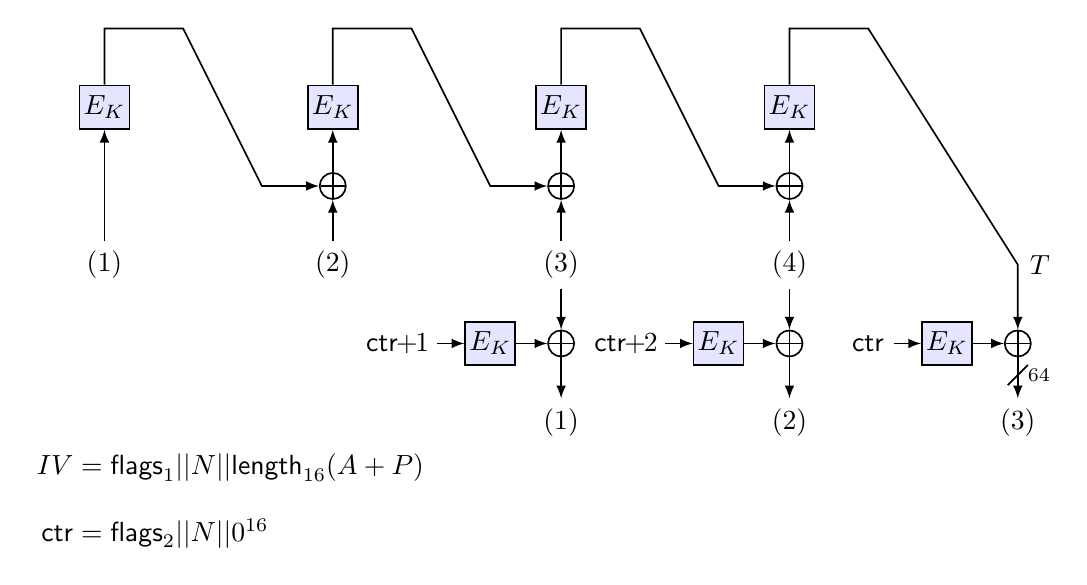
\begin{tikzpicture}[
		block/.style = {draw,fill=blue!10,inner xsep=1.5,inner ysep=3.7,align=center},
		XOR/.style = {draw,circle,append after command={
		     		   [shorten >=\pgflinewidth, shorten <=\pgflinewidth,]
		        			(\tikzlastnode.north) edge (\tikzlastnode.south)
		        			(\tikzlastnode.east) edge (\tikzlastnode.west)
		        }
		},
		every path/.style = {semithick},
		arrowstyle/.style = {->,>=latex},
	]
	
	\def\xspacesep{2.9}

	
%
%	\foreach \i in {1, ..., 30} {
%		\foreach \j in {1, ..., 10} {
%			\coordinate (d\i,\j) at (\i,\j);		
%		}
%	}
	
	\foreach \i in {1, ..., 4} {
		\node[block] (Eu\i) at (\xspacesep*\i - 2, 5) {$E_K$};
	}
	
	\foreach \i in {2, ..., 4} {
		\node[XOR] (Ou\i) at (\xspacesep*\i - 2, 4) {};
	}
	
	\foreach \i in {1, ..., 4} {
		\node (P\i) at (\xspacesep*\i - 2, 3) {\plaintext(\i)};
	}
	
	\foreach \i in {3, ..., 5} {
		\node[XOR] (Od\i) at (\xspacesep*\i - 2, 2) {};
	}
	

	
	\foreach \i in {1, ..., 3} {
		\node[block] (Ed\i) at (\xspacesep*\i + 2.9, 2) {$E_K$};
	}
	
	\foreach \i [count = \j from 3] in {1, ..., 3} {
		\node (C\i) at (\xspacesep*\j - 2, 1) {\ciphertext(\i)};
	}

	\foreach \i  in {1, 2} {
		\node[xshift=-5pt,left of=Ed\i] (ctr\i)  {$\mathsf{ctr} \hspace{-3pt} + \hspace{-3pt} \i$};
		\draw[arrowstyle] (ctr\i) + (0.5, 0) -- (Ed\i); 
	}

	
	\draw[arrowstyle] (P1) -- (Eu1);

	\foreach \i in {2, ..., 4} {
		\draw[arrowstyle] (P\i) -- (Ou\i);
		\draw[arrowstyle] (Ou\i) -- (Eu\i);
	}
	
	\foreach \i [count=\j from 2] in {1, ..., 3} {
		\draw[arrowstyle] (Eu\i) -- (\xspacesep*\i - 2,6) |- (\xspacesep*\i - 1, 6) -- (\xspacesep*\i, 4) -- (Ou\j); 
	}
	\draw[arrowstyle] (Eu4) -- (\xspacesep*4 - 2,6) |- (\xspacesep*4 - 1, 6) -- (\xspacesep*5 - 2, 3) -- (Od5); 
	
	
	\foreach \i [count=\j from 3] in {1,2} {
		\draw[arrowstyle] (P\j) -- (Od\j);
		\draw[arrowstyle] (Ed\i) -- (Od\j);
		\draw[arrowstyle] (Od\j) -- (C\i);
	}
	
	\node[left of=Ed3] (ctr0) {$\mathsf{ctr}$};
	\draw[arrowstyle] (ctr0) -- (Ed3); 
	\draw[arrowstyle] (Ed3) -- (Od5); 
	\draw[arrowstyle] (Od5) -- node[strike out,draw,-,yshift=1pt]{} node[right,yshift=1pt] {\scriptsize 64} (C3);	
	\node[above of = Od5, xshift=8pt] {$T$};
	

	\node[align=left] at (2.5,0) {
		$IV = \mathsf{flags}_1 || N || \mathsf{length}_{16}( A + P)$\\
		\\
		$\hspace{1.6pt} \mathsf{ctr} = \mathsf{flags}_2 || N || 0^{16}$ 
	};
	

	
\end{tikzpicture}


\end{document}